\onecolumn
\chapter{Maps} \label{maps}

\section{Tempestas}
\begin{center}
	\includegraphics[width=\linewidth]{img/Tempestas.jpg}
	
	{\textbf{Tempestas:} The main trading post of the south west region of the planet. Everything can be found here from crime, to various trade skills.}
\end{center}

\section{Aurushire}
\begin{center}
	\includegraphics[width=\linewidth]{img/Aurushire.png}
	
	{\textbf{Aurushire:} To the south is the sea entrance. In the northwest is a secluded area where Baba Lives. To the northeast is a secluded area where Belmod lives. The North path leads to The Pluvian Forest and the West path leads to Rem Silva. The East side of the village is the location of Auru Convallis and the Naga camps are on the southeast side of the area leading into the eastern forest.}
\end{center}

\section{Rem Silva}
\begin{center}
	\includegraphics[width=\linewidth]{img/RemSilva.png}
	
	{\textbf{Rem Silva:} A forest to the west of Aurushire. To the north/Northeast is The Pluvian Forest but the forest is too dense to travel between the two.}
\end{center}

\section{Spati Aethereu Thalamun}
\begin{center}
	\includegraphics[width=\linewidth]{img/Aethereu.png}	
	
	{\textbf{Aethereu:} The space chamber is composed of multi layered triangle rooms that can rotate about one another.}
\end{center}

\section{The Halls of No End}
\begin{center}
	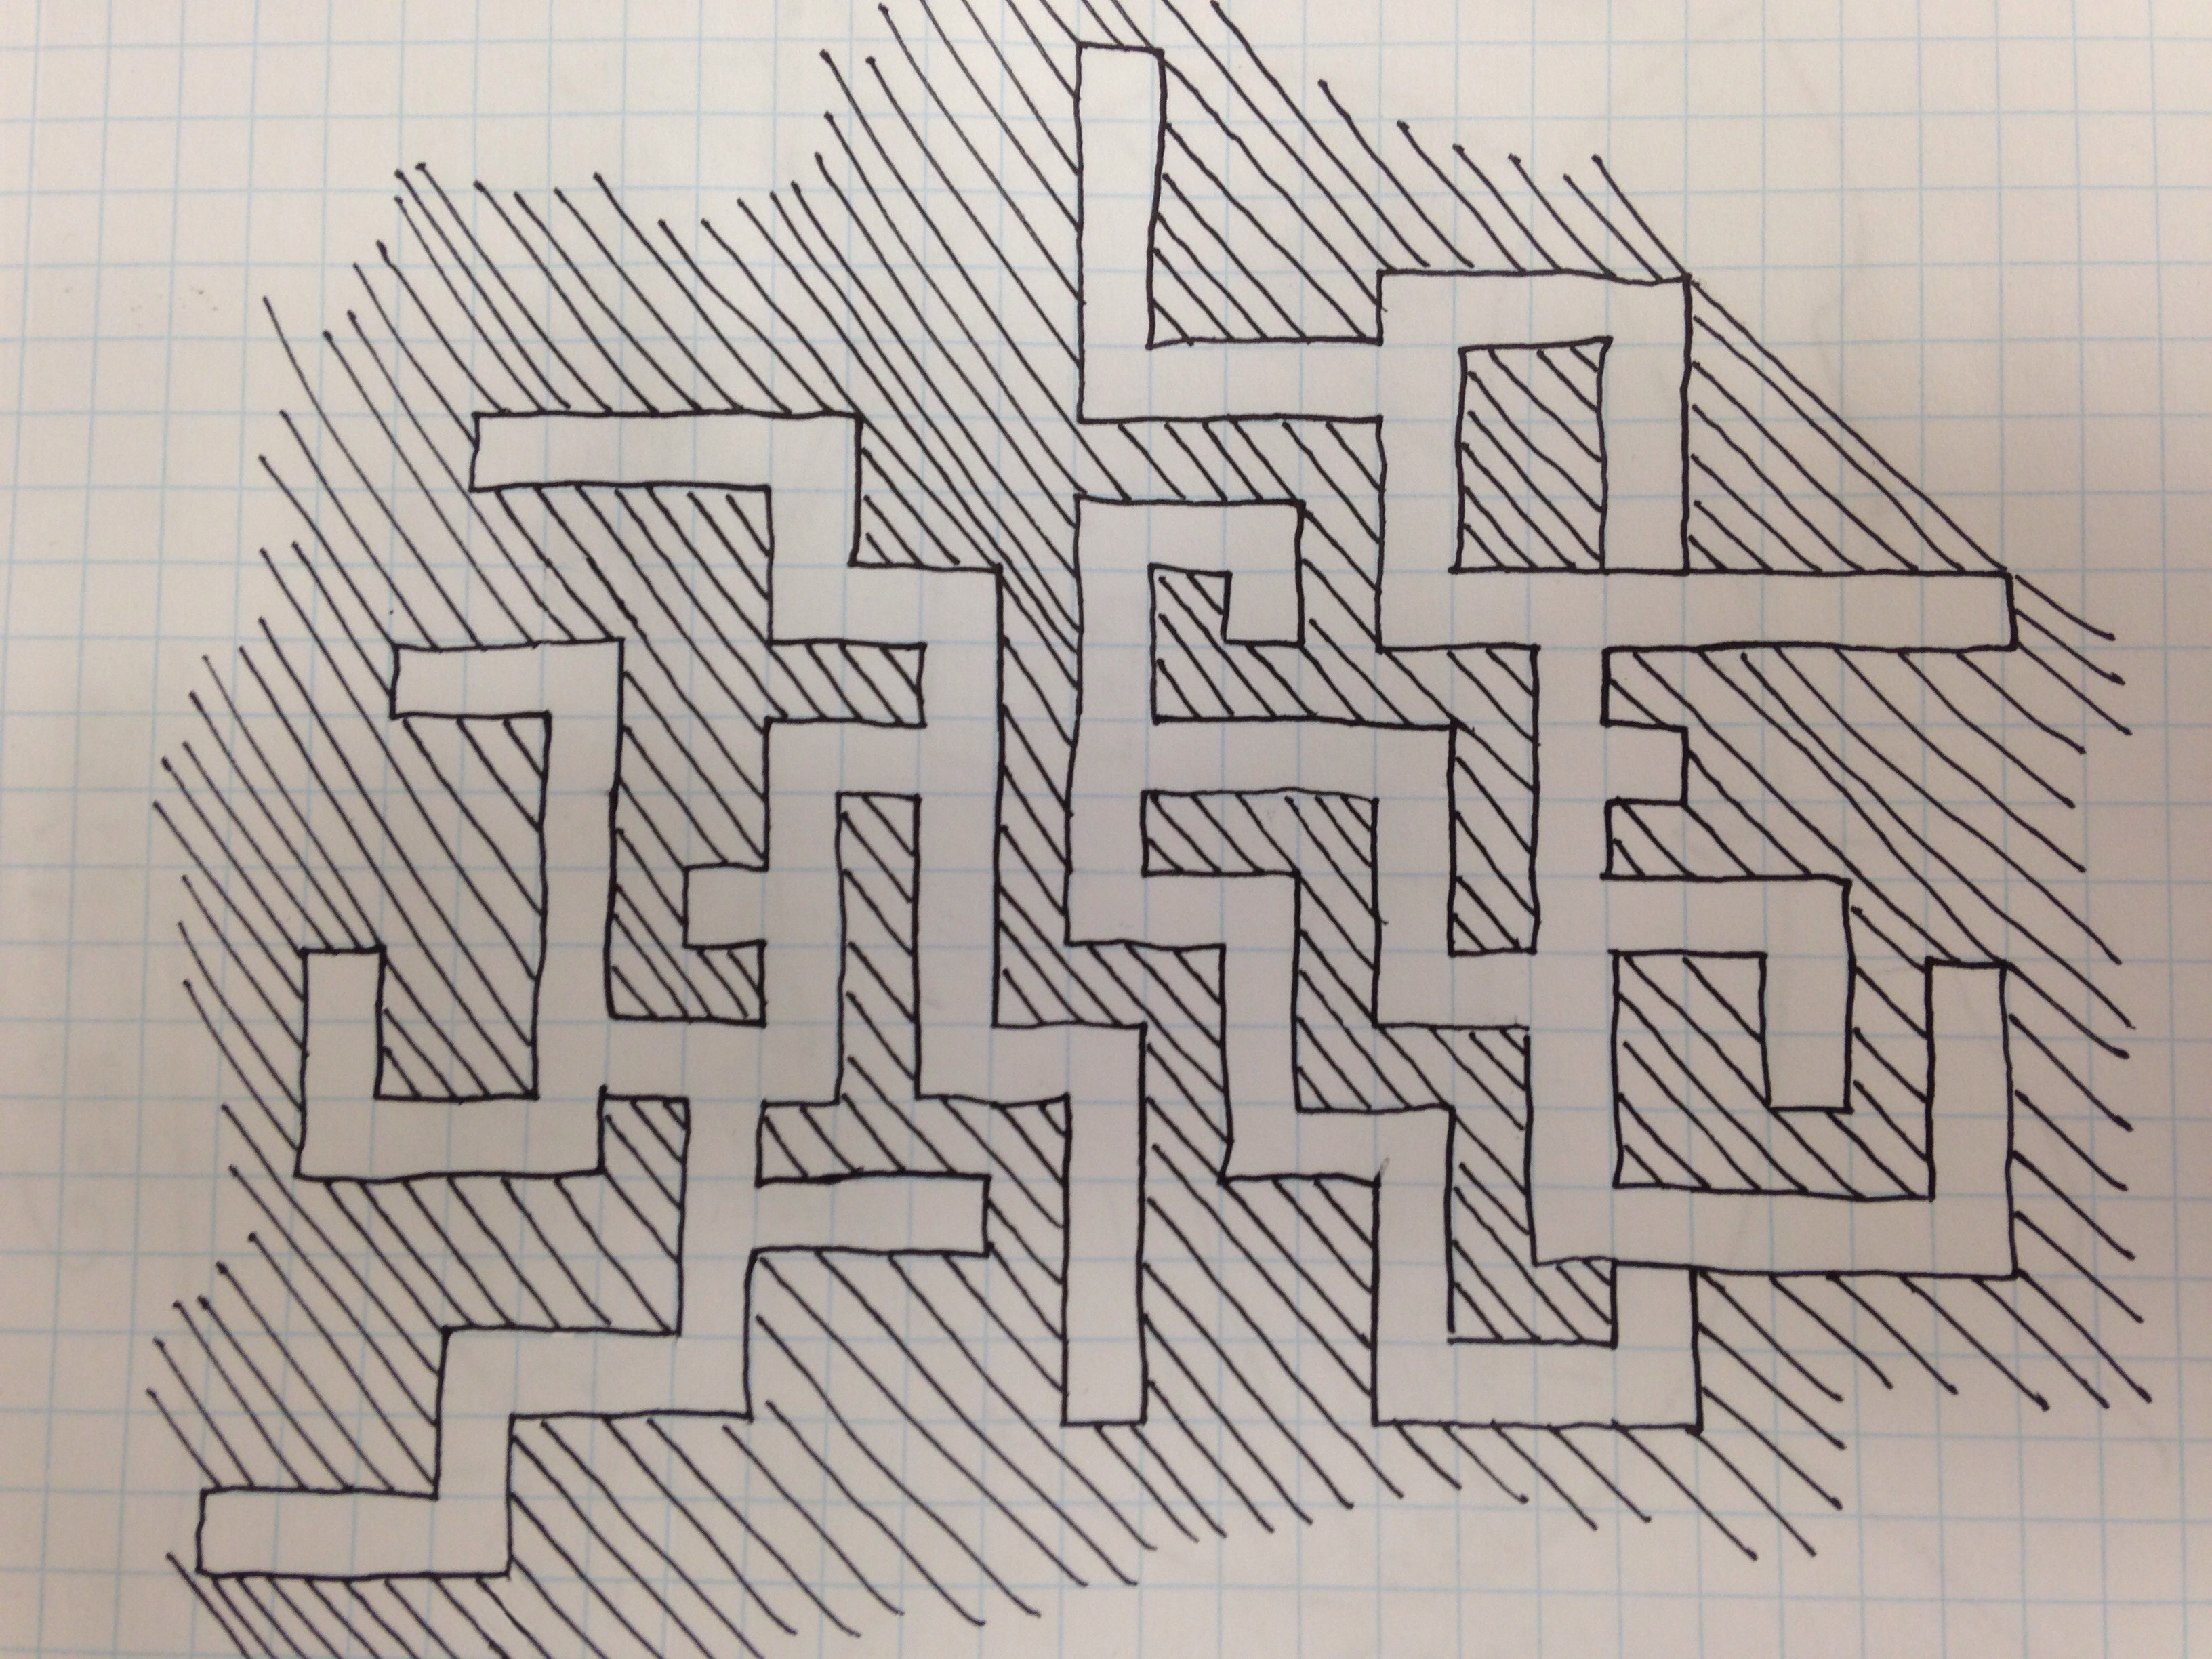
\includegraphics[width=\linewidth]{img/HONE.png} 
	
	{\textbf{Aethereu:} The Halls of no end is a puzzle area. There is one exit and it's the dead end which appears on the 2 long hallway to the left. Each hallway continues onto the hallway that is of the same length but opposite direction as it.}
\end{center}